\section{Uppgift 6}\label{sec:uppg06}

\subsection{Instruktioner}
\begin{verbatim}
6. Skriv ett program som räknar och skriver ut hur många förekomster det finns
   av vokalerna a, e, i, o, u och y i en sträng. Strängen ska matas in av den
   som kör programmet. Du ska deklarera en räknar-variabel för varje vokal och
   använda dig av en switch-sats.
   Exempel på körning:

        Mata in strängen: *Du har min kursbok*
        I strängen finns: 1 st a:n
        0 st e:n
        1 st i:n
        1 st o:n
        2 st u:n
        0 st y:n
\end{verbatim}


\subsection{Källkod}
\javacode{src/main/Lab2Uppg06.java}
\caption{Lab2Uppg06.java}
\label{src:uppg06}


\subsection{Skärmdump}
\begin{figure}[htbp]
    \centering
        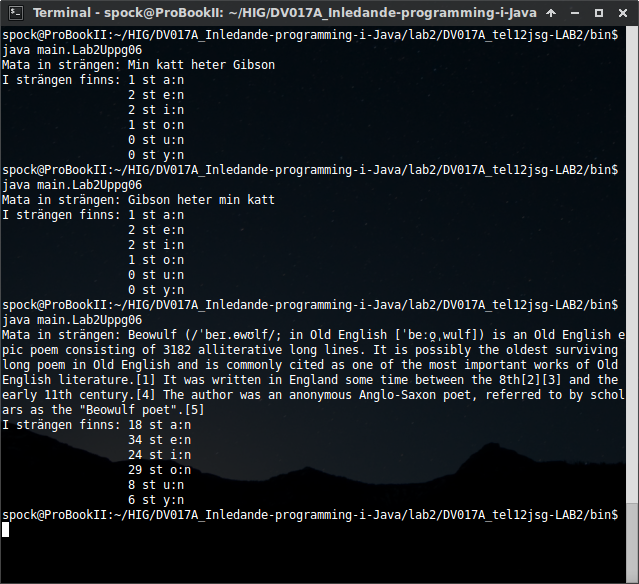
\includegraphics[width=\linewidth]{img/06.png}
    \caption{Körning av koden till Uppgift~\ref{sec:uppg06}}
    \label{fig:uppg06-screenshot}
\end{figure}

